\documentclass[12pt, 2024, professor]{uftpibic}

\usepackage[alf]{../abntex2/abntex2cite}
%\renewcommand{\backrefpagesname}{}
%\renewcommand{\backref}{}
\renewcommand*{\backrefalt}[4]{}
%\usepackage{cite}
\usepackage{tikz}
\usepackage{multirow}
\graphicspath{{}{images/}{figures/}} 
\usepackage{longtable}
\usepackage{amsmath,amssymb}

%% You can use these commands to check the CNPq option ----------%
\makeatletter
\newcommand{\ok}{\makebox[0pt][l]{(\ \ \ )}\raisebox{.15ex}{\hspace{0.1em}\color{blue}{ $\checkmark\quad$}}}
\newcommand{\ko}{\makebox[0pt][l]{(\ \ \ )}\raisebox{.15ex}{\hspace{0.1em}$\qquad$}}
\makeatother
%% --------------------------------------------------------------%
\usepackage[letterspace=-45]{microtype}

\usepackage{amsthm}

\theoremstyle{plain}
\newtheorem{thm}{Teorema}
\newtheorem{defn}{Definição} % definition numbers are dependent on theorem numbers
\newtheorem{lem}{Lema} % same for example numbers

%-------------------------------------------------------------------------------------------------------------------------%
% Endereço Institucional
%-------------------------------------------------------------------------------------------------------------------------%
\address{Quadra 109 Norte, Av. Ns 15, ALCNO 14, Bl 04, Sala 15, Propesq}
\cep{77001-090}
\phone{(63) 3229-4037 }
\mail{propesq@uft.edu.br}
\city{Palmas}
%-------------------------------------------------------------------------------------------------------------------------%
% Dados do Projeto
%-------------------------------------------------------------------------------------------------------------------------%
\title{Análise de correlação estatística entre dados da rede EMBRACE e imagens solares}
\advisor{Prof.}{Tiago da Silva}{Almeida}{Ms.}
\author{Caio Henrique}{Machado}
\campus{Campus Universitário de Palmas -- CUP}
\department{Ciência da Computação}
\local{Campus Universitário de Palmas -- CUP, Bloco III, Sala 107}
\area{Ciências Exatas e da Terra}
\financiamento{}
\grupo{GCC -- Grupo de Computação Cientifica}

\keyword{INPE}
\keyword{EMBRACE}
\keyword{Tempestade Solar}
\keyword{Redes Neurais Artificiais}
\keyword{Aprendizado de Máquina}
\keyword{Clima Espacial}

\equipeexecutora{Tiago da Silva Almeida}{Coordenador}
\equipeexecutora{Caio Henrique Machado}{Aluno}
%-------------------------------------------------------------------------------------------------------------------------%
% Para evitar a quebra automática dos Capítulos, descomentar abaixo
%-------------------------------------------------------------------------------------------------------------------------%
\makeatletter
\patchcmd{\chapter}{\if@openright\cleardoublepage\else\clearpage\fi}{}{}{}
\makeatother
%-------------------------------------------------------------------------------------------------------------------------%
\begin{document}

\maketitle

\vspace{1cm}
\chapter{ENQUADRAMENTO CNP\lowercase{q}}

\onehalfspace
Conforme determinação do Conselho Nacional de Desenvolvimento Científico e Tecnológico (CNPq), para ser contemplado com bolsa fomentada pelo conselho, o projeto de pesquisa do orientador deve se enquadrar em uma das opções abaixo. Assinale o enquadramento de sua proposta de projeto de pesquisa:

\bigbreak

\ok \textbf{Opção 1}. Apresenta aderência a, no mínimo, uma das Áreas de Tecnologias Prioritárias do Ministério da Ciência, Tecnologia, Inovações e Comunicações (MCTIC), conforme estabelecido na Portaria MCTIC nº 1.122/2020, com texto alterado pela Portaria MCTIC nº 1.329/2020 (\url{www.mctic.gov.br/mctic/opencms/legislacao/portarias/Portaria_MCTIC_n_1122_de_19032020.html})

\bigbreak

\textbf{Assinale a (s) área (s) de enquadramento}:

\bigbreak

\ok  Tecnologias Estratégicas, nos seguintes setores: Espacial; Nuclear; Cibernética; e Segurança Pública e de Fronteira.

\ok Tecnologias Habilitadoras, nos seguintes setores: Inteligência Artificial; Internet das Coisas; Materiais Avançados; Biotecnologia; e Nanotecnologia.

\ko Tecnologias de Produção, nos seguintes setores: Indústria; Agronegócio; Comunicações; Infraestrutura; e Serviços.

\ko Tecnologias para o Desenvolvimento Sustentável, nos seguintes setores: Cidades Inteligentes e Sustentáveis; Energias Renováveis; Bioeconomia; Tratamento e Reciclagem de Resíduos Sólidos; Tratamento de Poluição; Monitoramento, prevenção e recuperação de desastres naturais e ambientais; e Preservação Ambiental.

\ko Tecnologias para Qualidade de Vida, nos seguintes setores: Saúde; Saneamento Básico; Segurança Hídrica; e Tecnologias Assistivas.

\bigbreak

\ko \textbf{Opção 2}. O projeto de pesquisa é da área básica, humanidades e/ou ciências sociais e contribui para o desenvolvimento das Áreas de Tecnologias Prioritárias do MCTIC.


Art. 2º. Parágrafo único: ``São também considerados prioritários, diante de sua característica essencial e transversal, os projetos de pesquisa básica, humanidades e ciências sociais que contribuam para o desenvolvimento das áreas definidas nos incisos I a V do caput''.(Parágrafo único acrescido pela \href{http://www.in.gov.br/en/web/dou/-/portaria-n-1.329-de-27-de-marco-de-2020-250263672}{Portaria MCTIC nº 1.329, de 27.03.2020})

\bigbreak

\ko \textbf{Opção 3}. O projeto de pesquisa é de área básica e/ou fundamental, em interação com a pós-graduação e grupos ou redes de pesquisa.

\bigbreak

\textbf{OBSERVAÇÃO}: Somente poderão ser contemplados com cotas fomentadas pelo CNPq (PIBIC/CNPq e PIBIC/AF) - caso sejam indicados para tais cotas, após a pontuação da produtividade do orientador - os projetos que assinalarem uma das opções acima (1 a 3). Para se inscrever na modalidade de bolsa PIBITI, o projeto deve se enquadrar nas opções 1 ou 2.

\bigbreak

\ko \textbf{Opção 4}. O projeto de pesquisa não se enquadra em nenhuma das opções 1 a 3.

\bigbreak

\textbf{OBSERVAÇÃO}: o projeto de pesquisa que se enquadrar na opção 4 será, preferencialmente, contemplado com cotas fomentadas pela UFT (PIBIC/UFT) (mesmo que sejam indicados para cota CNPq, após a pontuação da produtividade do orientador).
\bigbreak

\textbf{Justifique o enquadramento na Opção 4 (Preenchimento obrigatório):} 

\noindent\makebox[\linewidth]{\rule{\textwidth}{.5pt}}

\noindent\makebox[\linewidth]{\rule{\textwidth}{.5pt}}

\noindent\makebox[\linewidth]{\rule{\textwidth}{.5pt}}

\noindent\makebox[\linewidth]{\rule{\textwidth}{.5pt}}

\noindent\makebox[\linewidth]{\rule{\textwidth}{.5pt}}

%\onehalfspace
%\pagebreak
\vspace{2cm}
\setlength{\parindent}{1.5cm}
\chapter{Introdução}

A maioria das tempestades solares produzem apenas pequenas perturbações na Terra como pequenas variações momentâneas da alimentação das redes de energia elétrica, interferência na comunicação entre aparelhos eletrônicos, necessidade de novo traçado de rotas para aeronaves, perda de alguns satélites. 

Mas uma tempestade solar pode ter a capacidade de causar grandes desastres na Terra caso se torne maior. A tempestade solar de setembro de 1859, que ficou conhecida como \textit{Carrington Flare} (Labareda de Carrington) foi um exemplo \cite{Carrington2003}. Outro exemplo aconteceu em julho de 2000, quando o governo japonês lançou um satélite telescópio, parte do programa de astronomia de raios-x, que sofreu danos irreversíveis após ser pego por uma tempestade solar \cite{Dennis2000}.

Existem hoje dois sistemas de captura de informações relacionadas à influência solar na Terra e ao comportamento do sol: a Rede EMBRACE de Magnetômetros (EMBRACE MagNet) \cite{Denardini2015,Denardini2016,Denardini2018,Denardini2018b}, uma rede de sensores posicionados estrategicamente por toda a América Latina, comunicando-se também com sensores de iniciativas internacionais com o mesmo objetivo de captar informações espaciais; e os satélites posicionados orbitando a Terra, capturando dados através de sensores gerando imagens, no projeto de estudos solar da NASA, SOHO (\textit{Solar and Heliospheric Observatory}) \cite{Akmal2001}.

A previsibilidade dos dados é fundamental para o sistema de alertas de tempestade solares, já existente no Brasil, por meio da EMBRACE. Além de ser uma fonte de dados muito importante na pesquisa e entendimento dos fenômenos eletromagnéticos do nosso planeta e do sistema Solar, o qual não é profundamente entendido ainda.

Pensando nisso, indagamos se existe uma correlação estatística perceptível entre os dados coletados pela rede EMBRACE e pelos dados de satélite do projeto SOHO. Se houver essa correlação, prevemos ser possível fazer modelos preditivos com algum grau de confiabilidade, permitindo nos preparar para eventuais problemas. Uma vez que as tempestades solares viajam na velocidade da luz, levando em torno de oito minutos para chegar a Terra, oito muito minutos é pouco tempo para qualquer preparação.

Logo, o objetivo deste trabalho é demonstrar e mensurar com algum grau de confiabilidade a correlação entre os dados dos dois sistemas de captura de informações solares, utilizando um modelo de RNA (Redes Neurais Artificiais). 

Trata-se de um projeto e uma linha de pesquisa bastante inovadora, e, até onde se sabe, não existem trabalhos simulares a esse. Contudo, a metodologia que será empregada já foi avaliada, ou mesmo testada em diferentes modelos de correlação entre variáveis utilizando RNA e modelos estatísticos de inferência. 

Nesse segundo viés, \citeonline{KARIMI2012} desenvolveram um modelo híbrido, incluindo uma RNA de retropropagação e Algoritmo Genético (GA) para estimar a densidade de nanofluidos. O GA foi acoplado a RNA para otimizar os parâmetros da RNA e melhorar a precisão do modelo proposto. A densidade experimental de quatro nanofluidos na faixa de temperatura de 273 a 323 K com a fração de volume de nanopartículas de até 10\% foi examinada. Os resultados obtidos pelo modelo RNA-GA apresentaram boa concordância com os dados experimentais com desvio absoluto de 0,13\% e alto coeficiente de correlação ($R \geq 0,98$). 

\citeonline{MATA2011} discutiu o processamento paralelo da informação em RNA. Este estudo mostra uma comparação entre os modelos de regressão linear múltipla e RNA para a caracterização do comportamento de barragens sob cargas ambientais. Como exemplo, o deslocamento horizontal registrado por um pêndulo foi estudado em uma grande barragem de arco portuguesa. Os resultados deste estudo mostraram que os modelos RNA podem ser uma ferramenta a ser incluída nas avaliações do comportamento de barragens de concreto existentes.

A utilização de modelos de RNA para predição já é amplamente estudada na literatura, como por exemplo os trabalhos de: \citeonline{MAY2011}; \citeonline{AKRAMI2013}; \citeonline{ABBOT2014}; \citeonline{Zhang2014}; \citeonline{SEIFFERT2014}; \citeonline{TIAN2015}; \citeonline{MAROHASY2015}; \citeonline{ABBOT2017}; \citeonline{Fichou2018}; e  \citeonline{LEE2018}.


\vspace{1.5cm}
\chapter{Objetivos}

O objetivo deste trabalho é obter dados dos sistemas EMBRACE e SOHO de captura de informações solares e traçar um comparativo fazendo uso de RNA para averiguar a concordância entre as informações e estabelecer e mensurar um grau de confiabilidade dessa correlação. Os passos se darão da seguinte maneira:

\begin{itemize}
\item Estudar os principais índices de medição eletromagnética da Terra (índice $Pk$);
\item Estudar os principais modelos de RNA e Aprendizado Profundo aplicado ao problema e implementar o modelo mais eficaz;
\item Criar um modelo baseado em RNA tendo como dado de entrada as imagens solares;
\item Coleta e classificação dos dados;
\item Análise do grau de erro do modelo;
\item Quantificação de forma estatística por meio da correlação entre as variáveis;
\end{itemize}


\vspace{1.5cm}
\chapter{Metodologia}

\section{EMBRACE}

A rede EMBRACE é formada por magnetômetros de fluxo de três eixos, construído para medições de precisão compactas e de alto desempenho do vetor do campo magnético da Terra, com faixa total de $\pm$ 70000 nT e faixas dinâmicas de $\pm$ 250 nT, $\pm$ 1000 nT e $\pm$ 2500 nT cobrindo a amplitude das variações diurnas dos componentes magnéticos de baixa a alta latitude \cite{Denardini2015}. 

Ele pode ser alimentado por qualquer fonte de alimentação de 220/110 VCA ou $\pm$ 12 VCC, e as saídas estão na forma de três tensões analógicas de 0 a $\pm$ 2,5 VCC, proporcional aos três componentes do vetor magnético que ela é capaz de medir: horizontal (H), declinação (D) e vertical (Z), ou seja, coordenadas cilíndricas.  A taxa do módulo de aquisição de dados é de 20 bits e é definida em conjunto com a unidade de controle eletrônico e a saída de dados USB ou serial, dependendo do modelo. O software de aquisição e monitoramento de dados inclui tanto armazenamento de dados local e upload simultâneo para dois servidores diferentes de arquivamento de dados \cite{Denardini2015}. 

O principal interesse da rede EMBRACE é mostrar a variação do componente H sem considerar o campo principal, que é basicamente a variação do componente H e deduzir o valor da linha de base, que é reproduzido na forma,

\begin{eqnarray}
\Delta H_k (t) = H_k(t) - H_k(00 LT)
\label{eq:01}
\end{eqnarray}

\noindent em que $t$ é o tempo (de 00 h00 a 23 h59 tempo universal com passo de tempo de 1 min), $k$ é o código da estação magnética (números de estação 1, 2, 3 e assim por diante), $H(t)$ é a variação diária do componente horizontal e $00 LT$ corresponde à meia-noite local na estação magnética. Este método mostra o comportamento do componente H considerando as forças locais (radiação atmosférica ou solar) e externa (vento solar). Uma segunda maneira de obter a variação do componente H, também adequado para estudos do clima espacial, é definir $\Delta H$ de acordo com,

\begin{eqnarray}
\Delta H_N (t) = \frac{1}{N} \sum_{k=1}^{N} (H_k(t) - QDC_k(t))
\end{eqnarray}

\noindent em que $t$, $k$ e $H (t)$ são os mesmos definidos em (\ref{eq:01}), enquanto $N$ é o número de estação magnética compreendida na derivação, e a derivação é a variação diária do componente horizontal, $QDC (t)$ é a variação diária do componente horizontal médio mensal, adquirido durante os cinco dias mais calmos do mês (\textit{Quiet Day Curve}). Esse método selecionará o componente H considerando apenas a força externa (vento solar) quando a força local (radiação atmosférica ou solar) for removida subtraindo o QDC \cite{Denardini2018b}.


\section{Redes neurais artificiais e aprendizado}

A principal ferramenta usada para este projeto será uma RNA, e / ou suas variações. RNA são técnicas de aprendizado de máquina que simulam os mecanismos de aprendizado de organismos biológicos. O sistema nervoso humano contém células chamadas de neurônios que são conectados uns aos outros pelos axiomas e dentritos, e as regiões onde os axiomas e dentritos se conectam são chamadas de sinapses. A força entre as ligações sinápticas muda de acordo com estímulos externos, e é esta mudança que causa o aprendizado em organismos vivos. 

O mecanismo biológico é simulado em RNA, as quais contêm unidades computacionais a que também chamamos de neurônios. Neste projeto, os termos redes neurais e neurônios serão usados para referenciar os modelos artificiais. As unidades computacionais são conectadas umas as outras por pesos, os quais servem com o mesmo propósito que as intensidades das conexões sinápticas nos organismos biológicos. Cada informação fornecida a um neurônio é qualificada com um peso, o que afeta a função computada na unidade. 

A RNA computa as informações propagando os valores computados de um neurônio a outro usando os pesos das entradas como parâmetros. O aprendizado acontece ao que os valores dos pesos conectando os neurônios se modificam. As informações fornecidas à rede durante o treinamento servem como o estímulo externo do aprendizado, oferecendo exemplos de entradas e saídas da função a ser aprendida. 

Por exemplo, as informações de treinamento podem ser dados contendo representações de pixels de uma imagem, e a saída, etiquetas para classificação da imagem de acordo com o que ela representa. Essas informações de entrada e saída como treinamento são alimentadas à RNA para fazer futuras predições das saídas. A informação de treinamento fornece correção aos pesos da rede neural dependendo de quão boa foi a predição da saída. O objetivo de modificar os pesos das sinapses é de modificar a função para que as futuras predições sejam mais corretas em futuras iterações. 

Assim, os pesos são alterados cuidadosamente de uma forma matematicamente justificada para reduzir os erros. Após sucessivas correções e ajustes dos pesos entre os neurônios e muitos pares de entradas e saídas, a função computada pela rede neural é refinada para fornecer predições com maior acurácia. Assim, se uma RNA é treinada com muitas imagens diferentes de uma cadeira, eventualmente será capaz de reconhecer uma cadeira que nunca viu antes. 

A RNA mais simples é chamada de \textit{perceptron}. Essa RNA contém uma única camada de entrada e um nó de saída. A arquitetura básica do \textit{perceptron} é mostrada na Figura \ref{fig:neuron}. Considere uma situação em que cada instância de treinamento tenha a forma $(X, y)$, em que cada $X = [x_1,. . . x_d]$ contém $d$ variáveis de recurso e $y \in \left[-1, +1\right]$ contém o valor observado da variável de classe binária. Por ``valor observado'', nos referimos ao fato de que ele nos é fornecido como parte dos dados de treinamento, e nosso objetivo é prever a variável de classe para os casos em que não é observado \cite{Aggarwal2018}. 

\begin{figure}[!htpb]
    \centering
    \caption{Representação de neurônios artificiais}
    \includegraphics[width=.6\textwidth]{aneuron.jpeg}
    \label{fig:neuron}
\end{figure}

A camada de entrada contém $d$ nós que transmitem os $d$ \textit{features} (características) em $X = [x_1. . . x_d]$ com arestas de peso $W = [w_1. . . w_d]$ para um nó de saída. A camada de entrada não realiza nenhum cálculo por si só. A função linear $W \times X = \sum_{i = 1}^{d} w_ix_i$ é calculada no nó de saída. Posteriormente, o sinal desse valor real é usado para prever a variável dependente de $X$. 

A arquitetura do \textit{perceptron é mostrada na Figura \ref{fig:neuron}, na qual uma única camada de entrada transmite os recursos para o nó de }saída. As arestas da entrada até a saída contêm os pesos $w_1. . . w_d$ com o qual os recursos são multiplicados e adicionados no nó de saída. Posteriormente, a função de sinal é aplicada para converter o valor agregado em um rótulo de classe. A função de sinal serve como função de ativação. 

Diferentes opções de funções de ativação podem ser usadas para simular diferentes tipos de modelos usados no aprendizado de máquina, como regressão de mínimos quadrados com destinos numéricos, a máquina de vetores de suporte ou um classificador de regressão logística. A maioria dos modelos básicos de aprendizado de máquina pode ser facilmente representada como arquiteturas de RNA simples. É um exercício útil para modelar técnicas tradicionais de aprendizado de máquina como arquiteturas neurais, porque fornece uma imagem mais clara de como o aprendizado generaliza o aprendizado de máquina tradicional \cite{Aggarwal2018}.

A utilidade primária de todo modelo de RNA é sua habilidade de generalizar seu aprendizado a partir de dados de treinamento fornecidos para exemplos novos nunca vistos \cite{SandroSkansi2018}.


%% Aqui pode fazer um breve introdução sobre RNA e Deep Learning, busca algumas figuras mais genéricas, sobre o tema, qualquer artigo ou livro tem isso. E fala um pouco soubre o indice Pk (acho que tem no artigo do Clézio). Também é legal comentar um pouco sobre os pacotes TensorFlow e PyTorch. Até porque você vai usar um deles (não sei qual). Não precisa programar a RNA do zero (nem quero que você faça isso).

%\begin{figure}[!htpb]
%\centering
%\caption{Diagrama de fluxo de dados do módulo veicular, destacando os sub-módulos envolvidos e os canais de comunicação em cada etapa.}
%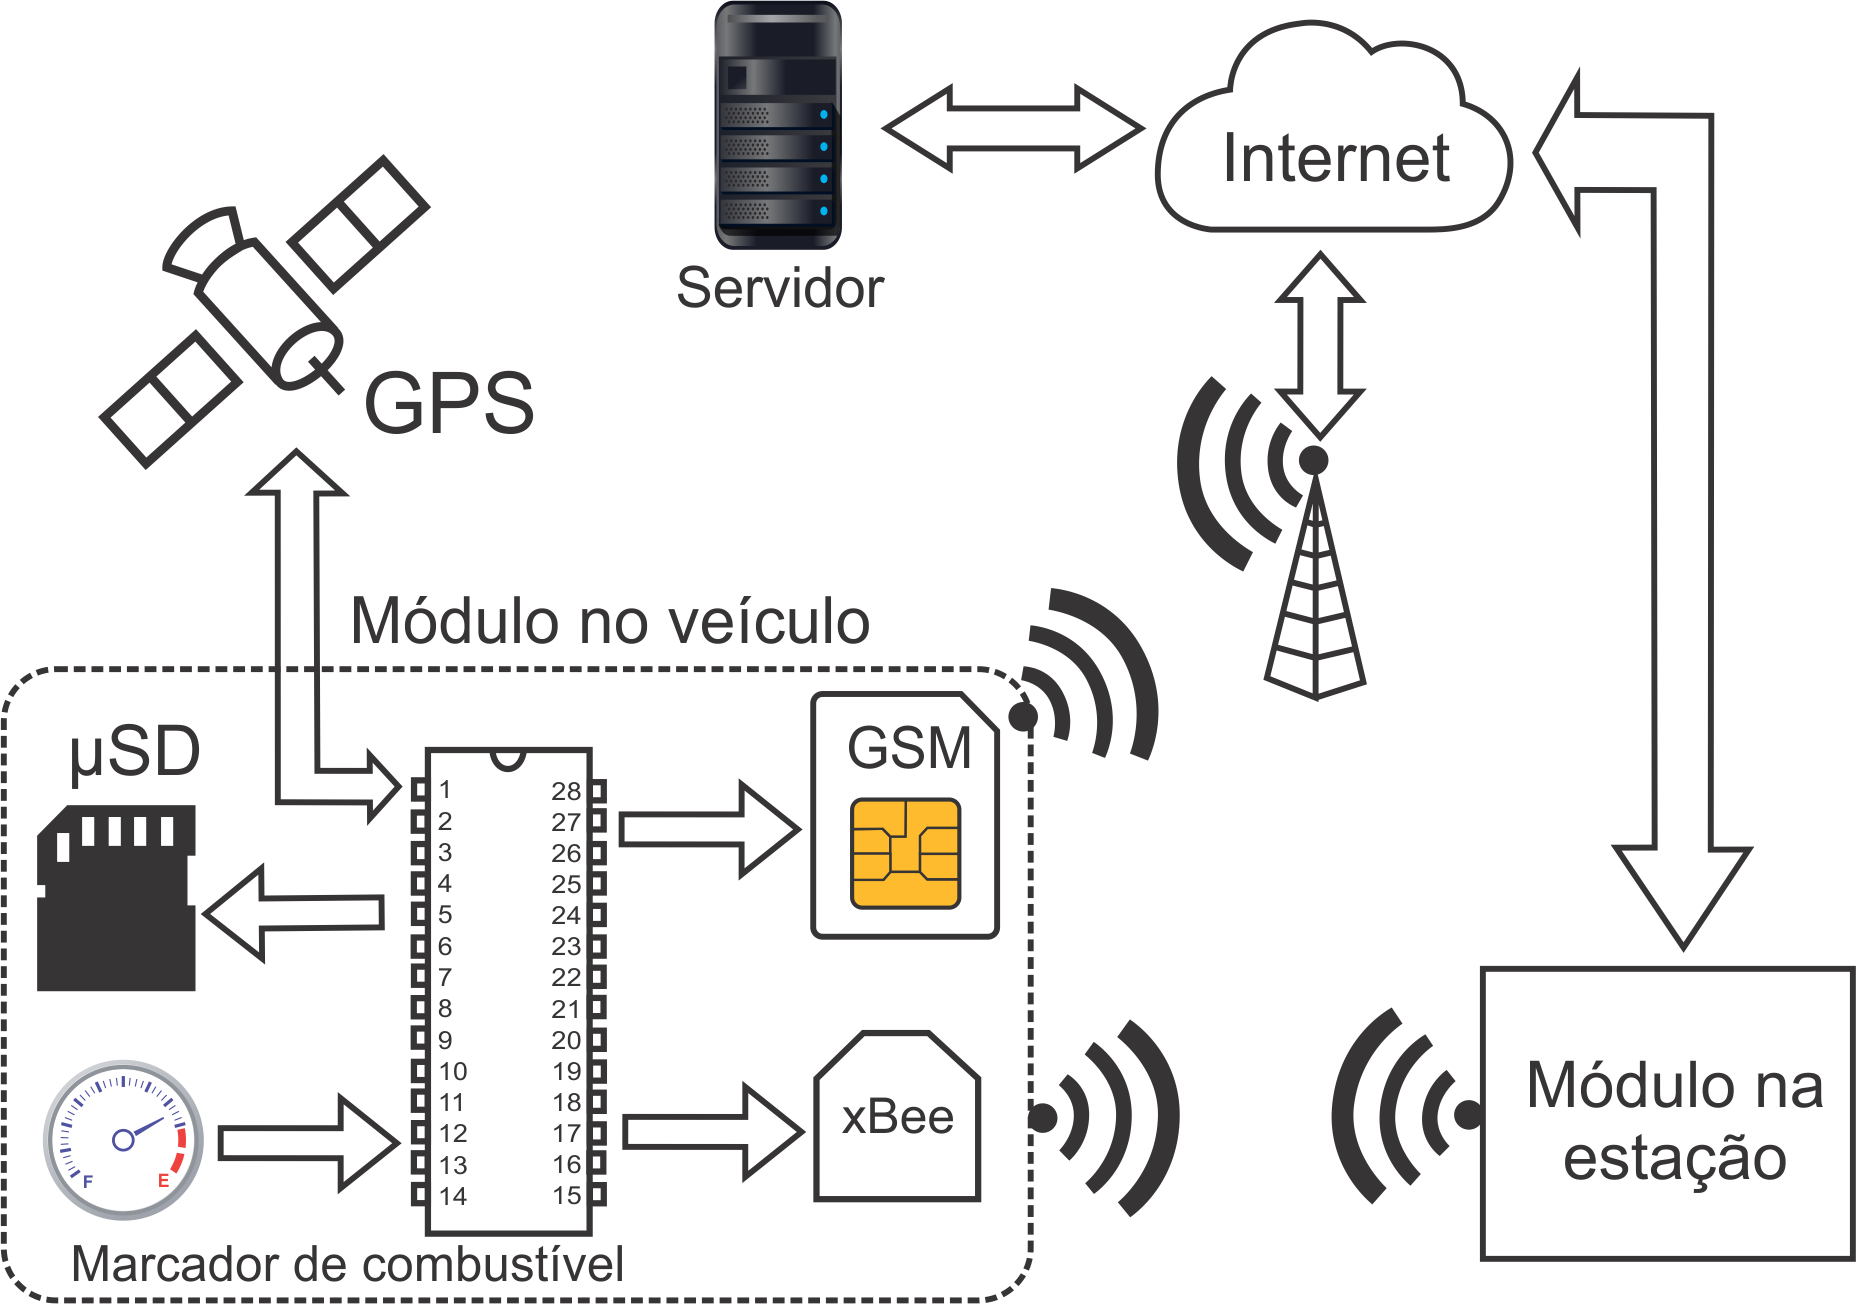
\includegraphics[scale=.8]{ruti1.png}
%\label{fig:projeto1}
%\end{figure}


\vspace{1.5cm}
\chapter{Cronograma de execução}

%% Ainda não corrigi, mas isso é rápido. Faço outra hora.
As atividades do trabalho são divididas conforme a Tabela \ref{tb:atividades}, enumeradas de A à J, e sua execução é de acordo com o cronograma da Tabela \ref{tb:cronograma}.

\begin{table}[!h]
  \centering
  \caption{Lista de atividades previstas.}\label{tb:atividades}
  \begin{tabular}{cp{9.4cm}}
    \hline \hline &\\[-0.4cm]
    {\bf Atividades} & \multicolumn{1}{c}{\bf Descrição} \\
    \hline
    &\\[-0.4cm]
    \textbf{A} &  Estudo da teoria e prática de redes neurais artificiais. \\[0.2cm]
    \textbf{B} &  Desenvolvimento e treinamento de uma rede neural artificial.\\[0.2cm]
    \textbf{C} &  Estudo da teoria e prática de processamento de imagens e descretização das imagens dos satélites.\\[0.2cm]
    \textbf{D} &  Alimentação da rede neural artificial com os dados das imagens e verificação de resultados. \\[0.2cm]
    \textbf{E} &  Aplicação e desenvolvimento de algoritmo de aprendizado de máquina. \\[0.2cm]
    \textbf{F} &  Coleta de dados da rede EMBRACE.\\[0.2cm]
    \textbf{G} & Estudo e criação do modelo de inferência linear entre as variáveis de estudo.\\[0.2cm]
    \textbf{H} & Análise estatística dos resultados. \\[0.2cm]
    \textbf{I} &  Escrita de relatório parcial em forma de trabalhos parciais para publicação em congressos e/ou periódicos e como relatório de prestação de contas com os sistemas de gestão da UFT. \\[0.2cm]
    \textbf{J} &  Escrita de relatório final em forma de trabalhos parciais para publicação em congressos e/ou periódicos e como relatório de prestação de contas com os sistemas de gestão da UFT. \\[0.2cm]
    \hline \hline
  \end{tabular}
\end{table}


\begin{table}[!ht]
  \centering %\fontsize{8}{12}%\tiny
  \caption{Cronograma de Atividades.}\label{tb:cronograma}
  \begin{tabular}{|c|c|c|c|c|c|c|c|c|c|c|c|c|}
    \hline
    {\normalsize\bf Ano}  &\multicolumn{12}{c|}{\normalsize\bf 2020/2021}\\
    \hline
 {\normalsize\bf Mês} &
\multirow{2}*{\bf Jul}&\multirow{2}*{\bf Ago}&\multirow{2}*{\bf Set}&\multirow{2}*{\bf Out}&\multirow{2}*{\bf Nov}&\multirow{2}*{\bf Dez}&
\multirow{2}*{\bf Jan}&\multirow{2}*{\bf Fev}&\multirow{2}*{\bf Mar}&\multirow{2}*{\bf Abr}&\multirow{2}*{\bf Mai}&\multirow{2}*{\bf Jun} \\
   \cline{1-1}
{\bf Atv.}    & & & & & & & & & & & &   \\
\hline
{\normalsize\bf A} & $\surd$ & $\surd$ & & & & & & & & & &  \\
\hline
{\normalsize\bf B} & & $\surd$ & $\surd$ & $\surd$ & $\surd$ & $\surd$ & $\surd$ & & & & & \\
\hline
%\hhline{>{\arrayrulecolor{black}}---->{\arrayrulecolor{black}}->{\arrayrulecolor{black}}------}
{\normalsize\bf C} & & & $\surd$ & $\surd$ & $\surd$ & $\surd$ & $\surd$ & & & & &  \\
%\hhline{>{\arrayrulecolor{black}}----->{\arrayrulecolor{black}}-->{\arrayrulecolor{black}}----}
\hline
{\normalsize\bf D} & & & & & $\surd$ & $\surd$ & $\surd$ & $\surd$ & $\surd$ & & &  \\
%\hhline{>{\arrayrulecolor{black}}------>{\arrayrulecolor{black}}->{\arrayrulecolor{black}}----}
\hline
{\normalsize\bf E} & & & & & & $\surd$ & $\surd$ & $\surd$ & $\surd$ & $\surd$ & &  \\
%\hhline{>{\arrayrulecolor{black}}------->{\arrayrulecolor{black}}->{\arrayrulecolor{black}}---}
\hline
{\normalsize\bf F} & & & & & & & $\surd$ & $\surd$ & $\surd$ & $\surd$ & $\surd$ & \\
% \hhline{>{\arrayrulecolor{black}}-------->{\arrayrulecolor{black}}-->{\arrayrulecolor{black}}-}
\hline
{\normalsize\bf G} & & & & & & & & & $\surd$ & $\surd$ & $\surd$ &  \\
% \hhline{>{\arrayrulecolor{black}}-------->{\arrayrulecolor{black}}-->{\arrayrulecolor{black}}-}
\hline
{\normalsize\bf H} & & & & & & & & & & $\surd$ & $\surd$ & \\
% \hhline{>{\arrayrulecolor{black}}-------->{\arrayrulecolor{black}}-->{\arrayrulecolor{black}}-}
\hline
{\normalsize\bf I} & & & & & & $\surd$ & $\surd$ & &  & & &  \\
\hline

{\normalsize\bf J} & & & & & & & & & & & $\surd$ & $\surd$ \\
\hline
  \end{tabular}
\end{table}

\vspace{1.5cm}
\chapter{Resultados esperados}

%% Aqui já seria legal explicar bem o modelo de teste de hipóteses. Isso é encontrado em qualquer artigo de RNA ou livro de estatíticas. Pega o modelo, coloca as fórmulas e explica como será aplicado.

Ao final do projeto, esperamos demonstrar e mensurar a confiabilidade da correlação entre as informações de ambos os sistemas EMBRACE e imagens por satélites da base SOHO, além de podermos predizer em séries temporais os dados da rede EMBRACE a partir das imagens de satélite conhecendo o grau de confiabilidade da correlação.

Como as imagens da base SOHO ou mesmo os dados da rede EMBRACE podem apresentar erros de leitura. O ajuste desse modelo estatístico fará uso do método dos mínimos quadrados. Quando cada observação de um experimento é um par de números, geralmente é importante tentar prever um dos números do outro. Os mínimos quadrados são um método para construir um preditor de uma das variáveis a partir da outra, utilizando uma amostra de pares observados.

Estamos interessados em aprender sobre a distribuição condicional de alguma variável $Y$ (valor do índice $Pk$) para determinados valores de outras variáveis $X_1,. . . X_k$ (dados das imagens). As variáveis $X_1,. . . , X_k$  podem ser variáveis de controle cujos valores devem ser escolhidos (leitura das imagens). Em geral, algumas dessas variáveis podem ser aleatórias e outras podem ser variáveis de controle. Começamos com alguma terminologia \cite{degroot2012}.

\begin{defn}
\textbf{Regressão}. As variáveis $X_1,. . . , X_k$ são chamados de preditores e a variável $Y$ é chamada de resposta. A expectativa condicional de $Y$ para determinados valores $x_1,. . . , x_k$ de $X_1,. . . , X_k$ é chamada a função de regressão de $Y$ em $X_1,. . . , X_k$, ou simplesmente a regressão de $Y$ em $X_1,. . . X_k$ \cite{degroot2012}.
\end{defn}

A regressão de $Y$ em $X_1,. . . , X_k$ é uma função dos valores $x_1,. . . , x_k$ de $X_1,. . . X_k$. Nos símbolos, essa função é $E (Y | x_1,..., X_k)$. Assumiremos que a função de regressão $E (Y | x_1,.., X_k)$ é uma função linear com a seguinte forma,

\begin{eqnarray}
E(Y|x_1, . . . , x_k) = \beta_0 + \beta_1x_1 + . . . + \beta_kx_k
\end{eqnarray}

Os coeficientes $\beta_0,. . . , \beta_k$ são chamados de coeficientes de regressão. Suponhamos que esses coeficientes de regressão sejam desconhecidos. Portanto, eles devem ser considerados parâmetros cujos valores devem ser estimados. Vamos supor também que $n$ vetores de observações sejam obtidos (imagens). Para $i = 1,. . . , n$, assumiremos que o i-ésimo vetor ($x_{i1},..., x_{ik}, y_i$) consiste em um conjunto de valores controlados ou observados de $X_1,. . . , X_k$ e o valor observado correspondente de $Y$.

Um conjunto de estimadores dos coeficientes de regressão $\beta_0,. . . , \beta_k$ que pode ser calculado a partir dessas observações é o conjunto de valores $\widehat{\beta_0},. . . , \widehat{\beta_k}$ que são obtidos pelo método dos mínimos quadrados. Esses estimadores são chamados estimadores de mínimos quadrados de $\beta_0,. . . , \beta_k$. 

Consideraremos um problema no qual desejamos estudar a regressão de $Y$ em apenas uma única variável $X$. Assumiremos que para cada valor $X = x$, a variável $Y$ pode ser representada na forma $Y = \beta_0 + \beta_1x + \epsilon$, onde $\epsilon$ é uma variável aleatória que tem a distribuição normal com média 0 e variância $\sigma^2$. Segue-se desta suposição que a distribuição condicional de $Y$ dada $X = x$ é a distribuição normal com $\beta_0 + \beta_1x$ média e variância $\sigma^2$. Um problema desse tipo é chamado de problema de regressão linear simples. Aqui, o termo simples refere-se ao fato de que estamos considerando a regressão de $Y$ em apenas uma única variável $X$, em vez de em mais de uma variável; o termo linear refere-se ao fato de que a função de regressão $E (Y | x) = \beta_0 + \beta_1x$ é uma função linear dos parâmetros $\beta_0$ e $\beta_1$ \cite{degroot2012}.

Em particular, a junção condicional de $Y_1. . . Y_n$ é

\begin{eqnarray}
f_n(y|x, \beta_0, \beta_1, \sigma^2)=\frac{1}{(2\pi\sigma^2)^{n/2}}exp \left[-\frac{1}{2\sigma^2} \sum_{i=1}^{n} (y_i-\beta_0-\beta_1x_i)^2 \right]
\end{eqnarray}

Assim, é possível encontrar o MLE (\textit{Maximum Likelihood Estimation}, ou máxima verossimilhança) de $\beta_0$, $\beta_1$ e $\sigma^2$. E por fim, determinarmos a inferência linear sobre o modelo proposto.

\vspace{1.25cm}
\bibliography{bibliografia}

\end{document}



